%=========================================================================
%DADOS DA INSTITUIÇÃO
\logoInst{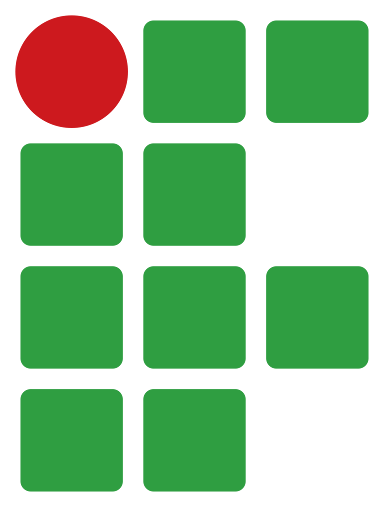
\includegraphics[width=0.4\textwidth]{./04-figuras/logoifba_capa}}

%======================================================================================================
%DADOS DO TRABALHO
%************************************************************************************
\titulo{Aplicação de Controle Adaptativo para Minimização de Risco em Estratégias de Hedge de Derivativos em Mercados Incompletos}
\titleenglish{Application of Adaptive Control for Risk Minimization in Derivative Hedging Strategies in Incomplete Markets}
%\subtitulo{Subtítulo do trabalho}
\autor{Laís Lorrayne Lima Chaves}
\tipotrabalho{Monografia} %troque por Tese (Doutorado) para tese de doutorado ou monografia se for o caso
\preambulo{Trabalho de Conclusão de Curso apresentado ao Instituto Federal de Educação, Ciência e Tecnologia de São Paulo como requisito parcial para obtenção do grau de Bacharel em Engenharia de Controle e Automação.}
%===============================================================
%ORIENTAÇÃO DO TRABALHO
%*****************************************************************
%\orientador{Prof. Me. Fulano de tal}  %Para orientadora:\orientador[Orientadora:]{Nome da orientadora}
%\coorientador{Prof. Dr. Sicrano Beltrano} %para coorientadora: \coorientador[Coorientadora:]{Nome da coorientadora}. Caso  tenha coorientador, descomente esta linha
\instCoorientador{Instituto Federal de Educação, Ciência e Tecnologia de São Paulo (IFSP)} %Necessário, pois o Coorientador pode ser de outra instituição (caso não seja, comente esta linha)
%\areaconcentracao{Modelagem Matemática e Computacional} %Não necessário no modelo 	UESC
%\linhapesquisa{Sistemas Inteligentes} %Não necessário no modelo UESC (caso necessário na sua intituição, descomente)
%========================================================================================================

%======================================================================================================
%DADOS DA INSTITUIÇÃO
%****************************************************************************************************
\instituicao{Instituto Federal de Educação, Ciência e Tecnologia de São Paulo (IFSP)} %instituição
\campus{CAMPUS SÄO PAULO} % Se não tiver, deixe em branco
\curso{GRADUAÇÃO EM ENGENHARIA DE CONTROLE E AUTOMAÇÄO} %caso não queira colocar deixe em branco dentro das chaves
\programa{} %PARA PROGRAMAS DE PÓS GRADUAÇÃO-Especialização, mestrado ou doutorado. Por exemplo: Programa de Pós Graduação em Modelagem Computacional Em Ciência e Tecnologia
\local{Säo Paulo - SP} %coloque o nome da cidade da sua instituição
\data{2025} %ano de defesa
%========================================================================================================

%======================================================================================================
%DADOS DA DEFESA
%****************************************************************************************************
%caso você não tenha coorienador comente a linha 38 do arquivo folhaAprovacao na pasta 01-Elementos-pre-textuais
%\datadefesa{04/08/2025} %Coloque  data de defesa

%\bancamembrointerno{Prof. Dr. Membro Interno} %Coloque o nome do membro interno que fará parte da banca
%\bancainstmembrointerno{IFBA} %Coloque o nome ou sigla da instituição do membro interno que fará parte da banca

%\bancamembroexterno{Prof. Me. Membro Externo} %Coloque o nome do membro externo que fará parte da banca
%\bancainstmembroexterno{UESB} %Coloque o nome ou sigla da instituição do membro externo que fará parte da banca

